
在这一章中，我们将定义、构造并研究\trPseudogradient{}场，其\trTrajectory{}连接着一个\trMorseFunction{}的诸\trCriticalPoint。这些\trVectorField{}使我们能够定义诸\trCriticalPoint{}的\trStableManifold{}与\trUnstableManifold，而它们将扮演重要的角色。我们提请读者注意“\trSmale{}性质”：例如，多亏了这一性质，连接两个\trIndex{}相继的\trCriticalPoint{}的\trTrajectory{}只有有限多条；我们还将证明满足该性质的\trPseudogradient{}场的存在性。

\section{\trGradient、\trPseudogradient{}与\trMorseChart}
\label{sec:gradients-pseudo-charts}\BookIndexDefinition{trPseudogradient}

\subsection{\trGradient{}与\trPseudogradient}
\label{subsec:gradients-and-pseudo-gradients}

如果 $f$ 是一个定义在 $\RR^n$ 上的函数，那么我们都熟悉它的\textbf{\trGradient}（gradient），亦即\trVectorField{} $\operatorname{grad}f$，它在 $\RR^n$ 的\trCanonical{}基下的坐标为
\[
\operatorname{grad}_x f=\Bigl(\frac{\partial f}{\partial x_1},\dotsc,\frac{\partial f}{\partial x_n}\Bigr)\text{，}
\]
或者更简洁地，它（也）是由下式定义的那个\trVectorField：
\[
\langle\operatorname{grad}_x f,Y\rangle=(df)_x(Y)
\]
其中 $Y\in\RR^n$ 是任意一个向量（当然，这里的尖括号 $\langle\ ,\ \rangle$ 表示 $\RR^n$ 中通常的\trEuclidean{}\trInnerProduct）。这个\trVectorField{}最重要的几条性质，都源于这样一个事实：这个\trInnerProduct{}是一个\trPositiveDefinite{}的\trSymmetricBilinearForm：
\begin{enumerate}[label=(\arabic*)]
\item 它恰好在函数 $f$ 的诸\trCriticalPoint{}处才为零；
\item 函数 $f$ 沿 $-\operatorname{grad}f$ 这个场的\trFlowLine{}是递减的：
\[
\frac{d}{ds}\bigl(f(\varphi^s(x))\bigr)=-\bigl\|\operatorname{grad}_{\varphi^s(x)}f\bigr\|^2<0\text{。}
\]
\end{enumerate}

\begin{remark}\label{thm:riemannian-gradient}
更一般地，如果给\trManifold{} $V$ 赋予一个\textbf{\trRiemann\trMetric}（Riemannian metric）（参见\cref{sec:riemannian-metrics-exp}），那么 $V$ 上的函数便有一个由同一公式
\[
\langle\operatorname{grad}_x f,Y\rangle=(df)_x(Y)
\]
（对每个 $Y\in T_xV$）所定义的\trGradient。
\end{remark}

\begin{remark}\label{thm:negative-gradient-convention}
毫无疑问，“流”与“高度”这两个词的联手，正是（如果我们可以斗胆这么说的话）使用负\trGradient{}这一（新近的）传统的源头：流是向下运动的。我们遵从了这个惯例，[66] 与 [49] 亦然，而 [46] 则不然。
\end{remark}

\begin{quote}
设 $f\colon V\to\RR$ 是一个\trManifold{}上的\trMorseFunction。一个\textbf{\trAdapted}（adapted）于 $f$ 的\textbf{\trPseudogradient{}场}（pseudo-gradient field）或\textbf{\trPseudogradient}（pseudo-gradient），是 $V$ 上的一个满足如下条件的\trVectorField{} $X$：
\begin{enumerate}[label=(\arabic*)]
\item 我们有 $(df)_x(X_x)\le 0$，其中等号成立当且仅当 $x$ 是一个\trCriticalPoint；
\item 在一个\trCriticalPoint{}邻域内的\trMorseChart{}中，$X$ 与 $\RR^n$ 的\trCanonical\trMetric{}下的负\trGradient{}相重合。
\end{enumerate}
\end{quote}

\begin{remark}\label{thm:pseudogradient-particular}
\trPseudogradient{}是一类相当特殊的\trVectorField。至于那些不是\trPseudogradient{}的\trVectorField，可参见\cref{ex:ch02-10}。
\end{remark}

\subsection{\trMorseChart}
\label{subsec:morse-charts}

这个观念使我们能够通过指明一个\trPseudogradient{}场 $X$ 的诸\trTrajectory，来把诸\trMorseChart{}刻画得更加精确。例如，\cref{fig:max-min}便最终展示了极大点（左边）与极小点（右边）之间的差别。

\begin{figure}[htbp]
\centering
\begin{minipage}[b]{0.44\textwidth}
\centering
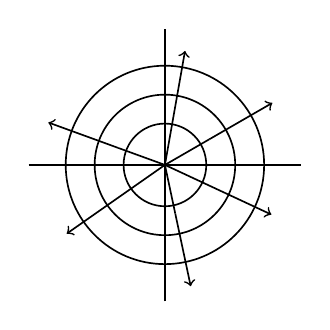
\begin{tikzpicture}[line width=0.6pt,scale=1.05]
  \draw (-1.65,0) -- (1.65,0);
  \draw (0,-1.65) -- (0,1.65);
  \draw (0,0) circle (0.5);
  \draw (0,0) circle (0.85);
  \draw (0,0) circle (1.2);
  \draw (80:0) -- (80:0.5); \draw[->] (80:0.5) -- (80:1.4);
  \draw (30:0) -- (30:0.62); \draw[->] (30:0.62) -- (30:1.5);
  \draw (-25:0) -- (-25:0.5); \draw[->] (-25:0.5) -- (-25:1.42);
  \draw (-78:0) -- (-78:0.6); \draw[->] (-78:0.6) -- (-78:1.5);
  \draw (215:0) -- (215:0.5); \draw[->] (215:0.5) -- (215:1.45);
  \draw (160:0) -- (160:0.6); \draw[->] (160:0.6) -- (160:1.5);
\end{tikzpicture}
\end{minipage}\hfill
\begin{minipage}[b]{0.44\textwidth}
\centering
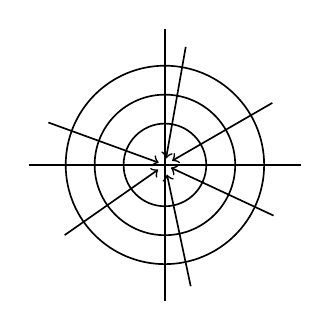
\begin{tikzpicture}[line width=0.6pt,scale=1.05]
  \draw (-1.65,0) -- (1.65,0);
  \draw (0,-1.65) -- (0,1.65);
  \draw (0,0) circle (0.5);
  \draw (0,0) circle (0.85);
  \draw (0,0) circle (1.2);
  \draw (80:1.45) -- (80:0.9); \draw[->] (80:0.9) -- (80:0.08);
  \draw (30:1.5) -- (30:1.0); \draw[->] (30:1.0) -- (30:0.1);
  \draw (-25:1.45) -- (-25:0.95); \draw[->] (-25:0.95) -- (-25:0.08);
  \draw (-78:1.5) -- (-78:1.0); \draw[->] (-78:1.0) -- (-78:0.12);
  \draw (215:1.48) -- (215:0.95); \draw[->] (215:0.95) -- (215:0.1);
  \draw (160:1.5) -- (160:1.0); \draw[->] (160:1.0) -- (160:0.08);
\end{tikzpicture}
\end{minipage}
\caption{极大点与极小点}
\label{fig:max-min}
\end{figure}

\cref{fig:morse-chart}展示了一个\trIndex{}为 $i$ 的\trCriticalPoint{}的一张\trMorseChart。这张\trChart——或者严格地说，是 $\RR^n$ 中的那个模型——出现在左边。在右边，我们可以看到它在\trManifold{}中的像（这里的函数是\trHeightFunction）。让我们固定一些记号。在 $\RR^n$ 中，\trQuadraticForm{} $Q$ 在一个 $i$ 维子空间 $V_-$ 上是\trNegativeDefinite{}的，而在 $V_+$ 上是\trPositiveDefinite{}的。我们令
\[
U(\varepsilon,\eta)=\bigl\{x\in\RR^n \bigm| -\varepsilon<Q(x)<\varepsilon \text{ 且 } \|x_-\|^2\|x_+\|^2\le\eta(\varepsilon+\eta)\bigr\}\text{。}
\]
既然我们是在 $\RR^n$ 中，函数 $Q$ 便有一个\trGradient，即
\[
-\operatorname{grad}_{(x_-,x_+)}Q=2(x_-,-x_+)\text{。}
\]
$U(\varepsilon,\eta)$ 的边界由三部分组成：
\begin{itemize}
\item $Q$ 的诸\trSublevelSet{}的两个子集：
\[
\partial_\pm U=\bigl\{x\in U \bigm| Q(x)=\pm\varepsilon \text{ 且 } \|x_\mp\|^2\le\eta\bigr\}\text{，}
\]
\footnote{译注：边界公式中的 $x\in U$ 按字面为空集（$Q(x)=\pm\varepsilon$ 与 $U$ 的定义 $-\varepsilon<Q(x)<\varepsilon$ 不容）；按后文的用法（$\partial_+U\cap V_+$ 径被用作 $V_+$ 中 $\|x_+\|^2=\varepsilon$ 的\trSphere）应理解作 $x\in\overline{U}$（或 $\partial U$）。此处照原书排印，存疑备案。——译者注}
\item \trGradient{} $\operatorname{grad}Q$ 的若干段\trTrajectory{}所成之集：
\[
\partial_0 U=\bigl\{x\in\partial U \bigm| \|x_-\|^2\|x_+\|^2=\eta(\varepsilon+\eta)\bigr\}\text{。}
\]
\end{itemize}
参见\cref{fig:morse-chart}。我们在此使用的记号取自 [46]。

\begin{figure}[htbp]
\centering
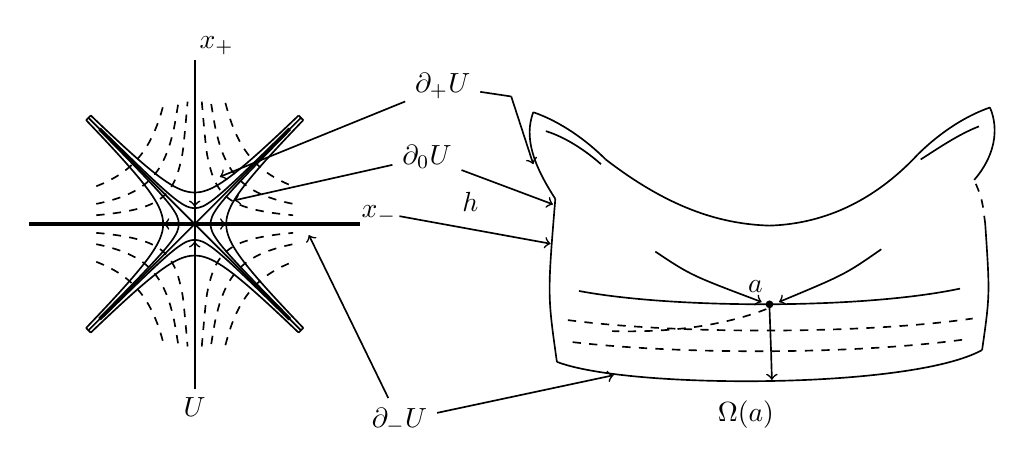
\begin{tikzpicture}[line width=0.6pt]
  \begin{scope}[shift={(0,0)}]
    \draw (0,-2.1) -- (0,2.08);
    \draw[line width=1.2pt] (-2.1,0) -- (2.1,0);
    \node at (0.28,2.26) {$x_+$};
    \node at (2.34,0.12) {$x_-$};
    \draw[domain=-1.32:1.32,samples=31,smooth] plot (\x,{sqrt(\x*\x+0.16)});
    \draw[domain=-1.32:1.32,samples=31,smooth] plot (\x,{-sqrt(\x*\x+0.16)});
    \draw[variable=\y,domain=-1.32:1.32,samples=31,smooth] plot ({sqrt(\y*\y+0.16)},\y);
    \draw[variable=\y,domain=-1.32:1.32,samples=31,smooth] plot ({-sqrt(\y*\y+0.16)},\y);
    \draw (0,0) -- (1.3493,1.3493);
    \draw (0,0) -- (-1.3493,1.3493);
    \draw (0,0) -- (1.3493,-1.3493);
    \draw (0,0) -- (-1.3493,-1.3493);
    \draw[domain=1.32:1.3792,samples=9,smooth] plot (\x,{1.8205/\x});
    \draw[domain=1.32:1.3792,samples=9,smooth] plot (\x,{-1.8205/\x});
    \draw[domain=-1.3792:-1.32,samples=9,smooth] plot (\x,{1.8205/\x});
    \draw[domain=-1.3792:-1.32,samples=9,smooth] plot (\x,{-1.8205/\x});
    \draw[domain=-1.2:1.2,samples=25,smooth] plot (\x,{sqrt(\x*\x+0.04)});
    \draw[domain=-1.2:1.2,samples=25,smooth] plot (\x,{-sqrt(\x*\x+0.04)});
    \draw[variable=\y,domain=-1.2:1.2,samples=25,smooth] plot ({sqrt(\y*\y+0.04)},\y);
    \draw[variable=\y,domain=-1.2:1.2,samples=25,smooth] plot ({-sqrt(\y*\y+0.04)},\y);
    \begin{scope}[dashed]
      \draw[domain=0.09:1.25,samples=21,smooth] plot (\x,{0.14/\x});
      \draw[domain=-1.25:-0.09,samples=21,smooth] plot (\x,{0.14/\x});
      \draw[domain=0.09:1.25,samples=21,smooth] plot (\x,{-0.14/\x});
      \draw[domain=-1.25:-0.09,samples=21,smooth] plot (\x,{-0.14/\x});
      \draw[domain=0.21:1.25,samples=21,smooth] plot (\x,{0.32/\x});
      \draw[domain=-1.25:-0.21,samples=21,smooth] plot (\x,{0.32/\x});
      \draw[domain=0.21:1.25,samples=21,smooth] plot (\x,{-0.32/\x});
      \draw[domain=-1.25:-0.21,samples=21,smooth] plot (\x,{-0.32/\x});
      \draw[domain=0.39:1.25,samples=21,smooth] plot (\x,{0.60/\x});
      \draw[domain=-1.25:-0.39,samples=21,smooth] plot (\x,{0.60/\x});
      \draw[domain=0.39:1.25,samples=21,smooth] plot (\x,{-0.60/\x});
      \draw[domain=-1.25:-0.39,samples=21,smooth] plot (\x,{-0.60/\x});
    \end{scope}
    \draw[->] (0,0.40) -- (0,0.22);
    \draw[->] (0,-0.40) -- (0,-0.22);
    \draw[->] (0.22,0) -- (0.40,0);
    \draw[->] (-0.22,0) -- (-0.40,0);
    \node at (0,-2.32) {$U$};
  \end{scope}
  \node (dplus) at (3.15,1.75) {$\partial_+U$};
  \draw[->] (dplus) -- (0.32,0.60);
  \draw (dplus) -- (4.02,1.62);
  \draw[->] (4.02,1.62) -- (4.30,0.76);
  \node (dzero) at (2.95,0.85) {$\partial_0U$};
  \draw[->] (dzero) -- (0.50,0.30);
  \draw[->] (dzero) -- (4.55,0.25);
  \draw[->] (2.60,0.10) -- (4.52,-0.25);
  \node at (3.50,0.28) {$h$};
  \node (dminus) at (2.60,-2.50) {$\partial_-U$};
  \draw[->] (dminus) -- (1.45,-0.14);
  \draw[->] (dminus) -- (5.32,-1.92);
  \begin{scope}[shift={(6.6,-0.3)}]
    \draw (-2.0,-1.45) .. controls (-1.1,-1.80) and (2.5,-1.80) .. (3.4,-1.30);
    \draw (-2.0,-1.45) .. controls (-2.12,-0.60) .. (-2.02,0.62);
    \draw (3.4,-1.30) .. controls (3.50,-0.60) .. (3.44,0.30);
    \draw[dashed] (3.44,0.30) .. controls (3.40,0.62) .. (3.30,0.86);
    \draw (-2.02,0.62) .. controls (-2.30,1.05) and (-2.42,1.40) .. (-2.30,1.72);
    \draw (-2.30,1.72) .. controls (-1.95,1.60) and (-1.62,1.36) .. (-1.38,1.12);
    \draw (-2.14,1.48) .. controls (-1.88,1.40) and (-1.62,1.22) .. (-1.44,1.06);
    \draw (3.30,0.86) .. controls (3.56,1.16) and (3.62,1.50) .. (3.50,1.78);
    \draw (3.50,1.78) .. controls (3.15,1.66) and (2.82,1.42) .. (2.58,1.18);
    \draw (3.36,1.54) .. controls (3.10,1.44) and (2.84,1.26) .. (2.62,1.12);
    \draw (-1.38,1.12) .. controls (-0.60,0.52) and (0.05,0.30) .. (0.70,0.28)
          .. controls (1.35,0.30) and (2.00,0.56) .. (2.58,1.18);
    \draw (-1.72,-0.55) .. controls (-0.50,-0.78) and (1.90,-0.78) .. (3.12,-0.52);
    \draw[->] (-0.75,-0.05) .. controls (-0.30,-0.35) .. (0.60,-0.69);
    \draw[->] (2.12,-0.02) .. controls (1.66,-0.34) .. (0.82,-0.69);
    \draw (0.70,-0.76) .. controls (0.71,-1.05) .. (0.72,-1.32);
    \draw[->] (0.72,-1.32) .. controls (0.73,-1.50) .. (0.73,-1.68);
    \begin{scope}[dashed]
      \draw (0.66,-0.78) .. controls (0.10,-1.00) and (-0.60,-1.08) .. (-1.30,-1.06);
      \draw (-1.86,-0.92) .. controls (-0.50,-1.10) and (1.90,-1.10) .. (3.28,-0.90);
      \draw (-1.80,-1.20) .. controls (-0.40,-1.36) and (1.80,-1.36) .. (3.22,-1.16);
    \end{scope}
    \fill (0.70,-0.72) circle (1.4pt);
    \node at (0.52,-0.50) {$a$};
    \node at (0.40,-2.12) {$\Omega(a)$};
  \end{scope}
\end{tikzpicture}
\caption{一张\trMorseChart}
\label{fig:morse-chart}
\end{figure}

\begin{remark}\label{thm:gradient-orthogonal-levels}
按照 $\RR^n$ 中\trGradient{}的定义，\trGradient{}的诸\trTrajectory{}与函数的诸\trLevelSet{}是\trOrthogonal{}的（\trLevelSet{}的\trTangentSpace{}正是函数\trDifferential{}的\trKernel）。因此，在\cref{fig:morse-chart}所示的模型中，它们以来自两个\trOrthogonal{}族的\trRectangularHyperbola{}的面貌出现，这就绝非偶然了。

细细察看这幅图的两个部分会很有用。在这两个部分中，我们都标出了\trCriticalLevel{}集（不妨就设它是水平 $0$）、两个正的\trRegular\trLevelSet{}与两个负的\trRegular\trLevelSet{}、界定\trChart{}的那些\trGradient{}\trTrajectory，以及终止或起始于\trCriticalPoint{}的那些负\trGradient{}\trTrajectory。

如果 $a$ 是函数 $f$ 的一个\trCriticalPoint，那么由\trMorseLemma，$a$ 的一个邻域可以被描述成某个 $U(\varepsilon,\eta)$ 在一个\trDiffeomorphism{} $h$ 下的像。我们将把这样一个邻域记作 $\Omega(a)$。我们也将写
\[
\partial_\pm\Omega(a)=h(\partial_\pm U)\text{，}\qquad \partial_0\Omega=h(\partial_0 U)\text{，}
\]
等等。正如\cref{fig:morse-chart}中那样，我们将尽量一致地使用下列记法：
\begin{itemize}
\item 用 $\Omega$ 表示诸\trChart{}的像（$\Omega$ 是\trManifold{}的一个子集）；
\item 用 $U$ 表示诸\trChart{}的定义域，即那些模型（$U$ 是 $\RR^n$ 的一个子集）。
\end{itemize}
\end{remark}

\subsection{\trPseudogradient{}场的存在性}
\label{subsec:existence-pseudogradients}

对于一切\trManifold{}上的一切\trMorseFunction，\trPseudogradient{}场都存在。例如，这是\trRiemann\trMetric{}存在性的一个推论；更确切地说，是在\trManifold{}的一个给定子集（诸\trCriticalPoint{}的一个邻域）上具有指定形式的\trRiemann\trMetric{}的存在性的一个推论。无论如何，它是\trPartitionOfUnity{}存在性的一个简单推论，我们马上就来表明这一点。

\begin{proof}[\trPseudogradient{}存在性的证明]
设 $c_1,\dotsc,c_r$ 是 $f$ 在\trManifold{} $V$ 上的诸\trCriticalPoint{}（其数目有限，因为 $V$ 是\trCompact{}的，而且\trMorseFunction{}的诸\trCriticalPoint{}都是\trIsolated{}的），并设 $(U_1,h_1),\dotsc,(U_r,h_r)$ 是这些点的邻域内的诸\trMorseChart。诸开像 $\Omega_j$ 当然被假定是两两不交的。我们再添上更多的集合，便得到 $V$ 的一个有限开\trCovering{} $(\Omega_j)_{1\le j\le N}$，它由诸\trChart{} $(U_j,h_j)$ 的开集的像构成。我们可以——而且我们也确实——假定：在这个\trCovering{}中，\trCriticalPoint{} $c_i$ 只包含在开集 $\Omega_i$ 之中。

对于定义在 $\RR^n$ 的一个\trOpen{}子集上的函数 $g$，我们以 $\operatorname{grad}g$ 表示它在 $\RR^n$ 的标准\trEuclidean\trMetric{}下的\trGradient。对每个下标 $j$，我们把 $\operatorname{grad}(f\circ h_j)$ 拉回到 $V$ 上，也就是说，用公式
\[
X_j(x)=-\bigl(T_{h_j^{-1}(x)}h_j\bigr)\bigl(\operatorname{grad}_{h_j^{-1}(x)}(f\circ h_j)\bigr)
\]
在开集 $\Omega_j$ 上定义一个\trVectorField{} $X_j$（这个公式看起来也许复杂，但这个对象本身却非常简单：我们取了函数 $f\circ h_j$ 的\trGradient——它是 $U_j$ 上的一个\trVectorField——并以自然的方式把它变换成了 $\Omega_j$ 上的一个\trVectorField）。直接由定义可知，在 $\Omega_j$ 上有 $X_j\cdot f\le 0$（这是负\trGradient{}的性质之一）。此外，$X_j$ 只在 $f$ 位于 $U_j$ 中的那个\trCriticalPoint{}处才为零（对 $j\le r$）。

接下来，我们利用与\trCovering{} $(\Omega_j)_j$ 相伴的\trPartitionOfUnity{} $(\varphi_j)_j$，把这些局部\trVectorField{} $X_j$ 延拓成定义在整个 $V$ 上的\trVectorField{} $\widetilde{X}_j$，即令
\[
\widetilde{X}_j(x)=
\begin{cases}
\varphi_j(x)X_j(x) & \text{若 } x\in\Omega_j\\
0 & \text{否则；}
\end{cases}
\]
最后一步是令
\[
X=\sum_{j=1}^{N}\widetilde{X}_j\text{。}
\]
不出所料，所得的\trVectorField{} $X$ 是一个\trAdapted{}于 $f$ 的\trPseudogradient，这是因为我们的确有
\[
(df)_x(X_x)=\sum_{j=1}^{N}(df)_x\bigl((\widetilde{X}_j)_x\bigr)\le 0\text{。}
\]
如果这个不等式取等号，那么对每个 $j$ 都有 $\varphi_j(x)X_j(x)=0$，于是要么 $x$ 是一个\trCriticalPoint，要么对每个 $j$ 都有 $\varphi_j(x)=0$（而这是荒谬的）。

设 $c_i$ 是 $f$ 的诸\trCriticalPoint{}之一。由构造，在“$U_i$ 除去其余诸开集 $U_j$ 之并后的余集”上，$X$ 与\trEuclidean\trGradient{}的像相重合；而这个余集是 $c_i$ 的一个邻域，它含有 $c_i$ 邻域内的一个小的\trMorseChart。
\end{proof}

\subsection{\trStableManifold{}与\trUnstableManifold}
\label{subsec:stable-unstable-submanifolds}

设 $a$ 是 $f$ 的一个\trCriticalPoint。以 $\varphi^s$ 表示某一个\trPseudogradient{}的\trFlow。我们定义它的\textbf{\trStableManifold}（stable manifold）为
\[
W^s(a)=\Bigl\{x\in V \Bigm| \lim_{s\to+\infty}\varphi^s(x)=a\Bigr\}
\]
并把它的\textbf{\trUnstableManifold}（unstable manifold）定义为
\[
W^u(a)=\Bigl\{x\in V \Bigm| \lim_{s\to-\infty}\varphi^s(x)=a\Bigr\}\text{。}
\]
在\cref{subsec:morse-charts}中所考虑的那种 $\RR^n$ 的\trOpen{}子集 $U=U(\varepsilon,\eta)$ 内，我们有
\[
W^s(0)=U\cap V_+ \qquad\text{以及}\qquad W^u(0)=U\cap V_-\text{。}
\]

在 \cref{subsec:morse-charts} 的记号下，$a$ 的\trStableManifold{}便是从 $h(U\cap V_+)=h(W^s(0))$ 与 $h(\partial_+U\cap V_+)\times\RR$ 之并出发，把边界上的点 $x$ 与 $s\ge 0$ 所对应的 $(x,s)$ 同 $\varphi^s(x)$ \trGluing{}而得到的。参见\cref{fig:stable-manifolds}。如果 $k$ 是\trCriticalPoint{} $a$ 的\trIndex，那么 $h(\partial_+U\cap V_+)$ 是一个维数为 $n-k-1$ 的\trSphere；它是在 $V_+$（一个维数为 $n-k$ 的\trVectorSpace）中的\trSphere{} $\|x_+\|^2=\varepsilon$ 在\trDiffeomorphism{} $h$ 下的像。

\begin{figure}[htbp]
\centering
\begin{tikzpicture}[line width=0.6pt]
  \begin{scope}[shift={(0,0.2)}]
    \draw[<->] (-1.18,0) -- (1.18,0);
    \draw (0,1.18) .. controls (0.17,0.17) .. (1.18,0);
    \draw (1.18,0) .. controls (0.17,-0.17) .. (0,-1.18);
    \draw (0,-1.18) .. controls (-0.17,-0.17) .. (-1.18,0);
    \draw (-1.18,0) .. controls (-0.17,0.17) .. (0,1.18);
    \draw (-0.5,2.15) .. controls (0.15,1.5) and (0.3,0.75) .. (0.17,0.06);
    \draw[->] (0.155,1.013) -- (0.212,0.586);
    \draw (0.17,0.06) .. controls (0.1,-0.45) and (0.12,-0.7) .. (0.18,-0.92);
    \draw[->] (0.3,-1.55) .. controls (0.2,-1.25) and (0.22,-1.1) .. (0.18,-0.92);
    \draw (0.3,-1.55) .. controls (0.45,-1.95) and (0.65,-2.1) .. (1.0,-2.25);
    \fill (0.17,0.06) circle (1.2pt);
    \node at (0.34,0.2) {$a$};
    \fill (0.3,-1.55) circle (1.2pt);
    \node at (0.62,-1.5) {$x$};
    \node at (-1.05,2.3) {$W^s(a)$};
    \node[anchor=west] at (0.27,-0.15) {$\varphi^s(x)$，$s\ge 0$};
    \node at (0.75,-2.5) {$\varphi^s(x)$，$s\le 0$};
  \end{scope}
  \begin{scope}[shift={(5.3,-0.4)}]
    \draw (0,0) ellipse (1.6 and 0.42);
    \draw (-1.6,0) .. controls (-1.2,-1.1) and (-0.6,-1.55) .. (0,-1.55)
          .. controls (0.6,-1.55) and (1.2,-1.1) .. (1.6,0);
    \draw[->] (0.52,2.0) .. controls (0.44,1.3) and (0.38,0.75) .. (0.35,0.4);
    \draw (0.35,0.4) .. controls (0.3,-0.3) and (0.22,-1.0) .. (0.06,-1.52);
    \node at (0.6,2.15) {$-\infty$};
    \node at (1.02,1.2) {$\RR$};
    \node at (0.72,0.32) {$0$};
    \node at (0.1,-1.85) {$+\infty$};
    \node at (2.25,0.3) {$S^{n-k-1}$};
    \node (ws) at (-2.45,-0.8) {$W^s(a)$};
    \draw[->] (ws) -- (-1.05,-0.62);
  \end{scope}
\end{tikzpicture}
\caption{\trStableManifold}
\label{fig:stable-manifolds}
\end{figure}

于是，诸\trStableManifold——同样地，还有诸\trUnstableManifold——都是\trSubmanifold：在\trCriticalPoint{}之外，\trStableManifold{}是\trEmbedding{} $(x,s)\mapsto\varphi^s(x)$ 的像；而在\trCriticalPoint{}的邻域内，它是 $V_+$ 的像。这个论证还表明，$W^s(a)$ \trDiffeomorphic{}于维数为 $n-k$ 的\trDisk{}（同样地，$W^u(a)$ \trDiffeomorphic{}于维数为 $k$ 的\trDisk）：$W^s(a)$ 可以通过添加唯一的“无穷远点”$a$，把 $S^{n-k-1}\times\RR$ \trCompactification{}而得到；它也是 $S^{n-k-1}\times\,]{-\infty},+\infty]$ 在“把\trSphere{} $S^{n-k-1}\times\{+\infty\}$ 等同于一个单独的点”这一等价关系下的商。

这样，我们便证明了下述结果。

\begin{proposition}\label{thm:stable-unstable-submanifolds}
\trCriticalPoint{} $a$ 的\trStableManifold{}与\trUnstableManifold{}是 $V$ 的、\trDiffeomorphic{}于开\trDisk{}的\trSubmanifold。此外，我们有
\[
\dim W^u(a)=\operatorname{codim}W^s(a)=\operatorname{Ind}(a)\text{。}
\]\noqed
\end{proposition}

这里，$\operatorname{Ind}(a)$ 表示点 $a$ 作为 $f$ 的\trCriticalPoint{}的\trIndex。

\emph{\trPseudogradient{}场的\trTrajectory。}

以 $\varphi^s_X$ 或 $\varphi^s$ 表示\trPseudogradient{} $X$ 的\trFlow。\trVectorField{} $X$ 的诸\trFlowLine{}或诸\trTrajectory{}最重要的性质是：它们全都连接函数 $f$ 的诸\trCriticalPoint——每条\trTrajectory{}都来自一个\trCriticalPoint{}并走向另一个\trCriticalPoint。

\begin{proposition}\label{thm:trajectories-connect-criticals}
我们假定\trManifold{} $V$ 是\trCompact{}的。设 $\gamma\colon\RR\to V$ 是\trPseudogradient{}场 $X$ 的一条\trTrajectory。那么，存在 $f$ 的两个\trCriticalPoint{} $c$ 与 $d$，使得
\[
\lim_{s\to-\infty}\gamma(s)=c \qquad\text{以及}\qquad \lim_{s\to+\infty}\gamma(s)=d\text{。}
\]
\end{proposition}

\begin{proof}
让我们证明：当 $t$ 趋于 $+\infty$ 时（举例来说），$\gamma(t)$ 有一个极限，并且这个极限是一个\trCriticalPoint。我们必须证明：$\gamma(t)$ 会到达某个\trCriticalPoint{} $d$ 的 $S_+(d)=\partial_+\Omega(d)\cap W^s(d)$。我们假设情形并非如此。那么，每当\trTrajectory{} $\gamma$ 进入一个\trMorse{}邻域，它随后必定也离开该邻域，并且由于 $f$ 沿 $\gamma$ 递减，它永远无法再回到这个邻域。设 $s_0$ 是 $\gamma$ 最后一次离开诸\trCriticalPoint{}的诸\trMorseChart{}之（有限）并
\[
\Omega=\bigcup_{c\in\operatorname{Crit}(f)}\Omega(c)
\]
（当然，$\operatorname{Crit}(f)$ 表示函数 $f$ 的\trCriticalPoint{}所成之集）的时刻。存在一个 $\varepsilon_0>0$ 使得
\[
\forall x\in V-\Omega\text{，}\quad (df)_x(X_x)\le-\varepsilon_0\text{。}
\]
从而，对每个 $s\ge s_0$，我们有
\[
\begin{aligned}
f(\gamma(s))-f(\gamma(s_0))
&=\int_{s_0}^{s}\frac{d(f\circ\gamma)}{du}\,du\\
&=\int_{s_0}^{s}(df)_{\gamma(u)}\bigl(X_{\gamma(u)}\bigr)\,du\\
&\le -\varepsilon_0(s-s_0)\text{，}
\end{aligned}
\]
于是
\[
\lim_{s\to+\infty}f(\gamma(s))=-\infty\text{，}
\]
而这是荒谬的。
\end{proof}

\subsection{\trSublevelSet{}的\trTopology：当我们不跨越\trCriticalValue{}时}
\label{subsec:sublevel-sets-no-crossing}

只要我们不跨越任何一个\trCriticalValue，诸\trLevelSet{}的\trTopology{}就不会改变。诸\trSublevelSet{}的\trTopology{}亦然。设
\[
V^a=f^{-1}\bigl(\,]{-\infty},a]\,\bigr)
\]
表示 $f$ 对应 $a$ 的\trSublevelSet。在\cref{subsec:regular-level-sets-sublevel-sets}中我们曾说过：如果 $a$ 是一个\trRegularValue，那么 $V^a$ 是一个\trManifoldWithBoundary。

\begin{theorem}\label{thm:sublevel-no-critical}
设 $a$ 与 $b$ 是两个实数，使得 $f$ 在区间 $[a,b]$ 内没有任何\trCriticalValue。我们再假定 $f^{-1}([a,b])$ 是\trCompact{}的。那么，$V^b$ \trDiffeomorphic{}于 $V^a$。
\end{theorem}

\begin{proof}
我们利用某个\trPseudogradient{} $X$ 的\trFlow{}把 $V^b$ 收缩到 $V^a$ 上。我们固定一个函数 $\rho\colon V\to\RR$，它取值
\[
\rho(x)=
\begin{cases}
-\dfrac{1}{(df)_x(X)} & \text{在 } f^{-1}([a,b]) \text{ 上}\\[2.5ex]
0 & \text{在该子集的一个\trCompact{}邻域之外，}
\end{cases}
\]
\trVectorField{} $Y=\rho X$ 在一个\trCompact{}集之外为零，从而它的\trFlow{} $\psi^s$ 对每个 $s\in\RR$ 都有定义。对一个固定点 $x\in V$，我们考察一元函数 $s\mapsto f\circ\psi^s(x)$。如果 $\psi^s(x)\in f^{-1}([a,b])$，那么我们有
\[
\frac{d}{ds}f\circ\psi^s(x)
=(df)_{\psi^s(x)}\Bigl(\frac{d}{ds}\psi^s(x)\Bigr)
=(df)_{\psi^s(x)}\bigl(Y_{\psi^s(x)}\bigr)
=-1\text{。}
\]
于是，对 $\psi^s(x)\in f^{-1}([a,b])$，我们有
\[
f\circ\psi^s(x)=-s+f(x)\text{。}
\]
由此可知，$V$ 的\trDiffeomorphism{} $\psi^{b-a}$ 把 $V^b$ 映到 $V^a$ 上。
\end{proof}

\begin{remark}\label{thm:deformation-retraction}
映射
\[
\begin{array}{rcl}
r\colon V^b\times[0,1] & \longrightarrow & V^b\\[0.5ex]
(x,s) & \longmapsto &
\begin{cases}
x & \text{若 } f(x)\le a\\
\psi^{s(f(x)-a)}(x) & \text{若 } a\le f(x)\le b
\end{cases}
\end{array}
\]
是 $V^b$ 到 $V^a$ 上的一个\textbf{\trDeformationRetract}（deformation retract）；也就是说，$r_0=\operatorname{Id}$，对所有 $t$，$r_t$ 在 $V^a$ 上都等于包含映射，而 $r_1$ 的像为 $V^a$。从而，$V^a$ 是 $V^b$ 的一个\trDeformationRetract{}核。
\end{remark}

\begin{corollary}[\trReeb{}定理]\label{thm:reeb-theorem}\BookIndexDefinition{T009}
设 $V$ 是一个\trCompact\trManifold。假定 $V$ 上存在一个只有两个\trCriticalPoint{}的\trMorseFunction。那么，$V$ \trHomeomorphic{}于一个\trSphere。
\end{corollary}

\begin{figure}[htbp]
\centering
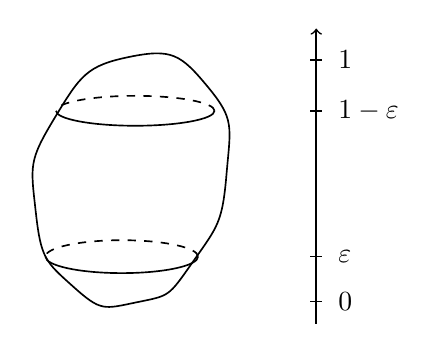
\begin{tikzpicture}[line width=0.6pt,scale=0.95]
  \draw plot [smooth cycle, tension=1] coordinates {(0,1.72) (1.05,1.32) (1.3,0.15) (0.85,-1.02) (0.1,-1.56) (-0.75,-1.35) (-1.25,-0.35) (-1.0,0.9)};
  \draw (-0.98,1.0) arc[start angle=180,end angle=360,x radius=1.06,y radius=0.2];
  \draw[dashed] (1.14,1.0) arc[start angle=0,end angle=180,x radius=1.06,y radius=0.2];
  \draw (-1.12,-0.95) arc[start angle=180,end angle=360,x radius=1.02,y radius=0.22];
  \draw[dashed] (0.92,-0.95) arc[start angle=0,end angle=180,x radius=1.02,y radius=0.22];
  \draw[->] (2.5,-1.85) -- (2.5,2.1);
  \draw (2.42,-1.55) -- (2.58,-1.55);
  \draw (2.42,-0.95) -- (2.58,-0.95);
  \draw (2.42,1.0) -- (2.58,1.0);
  \draw (2.42,1.68) -- (2.58,1.68);
  \node[anchor=west] at (2.66,-1.55) {$0$};
  \node[anchor=west] at (2.66,-0.95) {$\varepsilon$};
  \node[anchor=west] at (2.66,1.0) {$1-\varepsilon$};
  \node[anchor=west] at (2.66,1.68) {$1$};
\end{tikzpicture}
\caption{\trReeb{}定理}
\label{fig:reeb-theorem}
\end{figure}

\begin{proof}
这两个\trCriticalPoint{}必定是一个极小值和一个极大值。我们可以——而且我们也确实——假定 $f(V)=[0,1]$。于是，对充分小的 $\varepsilon>0$，\trMorseLemma{}断言 $f^{-1}([0,\varepsilon])$ 与 $f^{-1}([1-\varepsilon,1])$ 都是\trDisk{} $D^n$。由\cref{thm:sublevel-no-critical}，诸\trSublevelSet{} $V^{\varepsilon}$ 与 $V^{1-\varepsilon}$ 是\trDiffeomorphic{}的。于是，$V^{1-\varepsilon}$ 也是一个\trDisk{} $D^n$，而 $V$ 是两个沿着边界\trGluing{}的\trDisk{}之并。$V$ 这时\trHomeomorphic{}于一个\trSphere，这是一个经典结果：我们可以构造一个显式的映射
\[
h\colon D_1^n\cup_{\operatorname{Id}}D_2^n\longrightarrow D_1^n\cup_{\varphi}D_2^n
\]
即令
\[
h(x)=
\begin{cases}
x & \text{若 } x\in D_1^n\\
\|x\|\,\varphi\bigl(x/\|x\|\bigr) & \text{若 } x\in D_2^n-\{0\}\\
0 & \text{若 } x=0\in D_2^n\text{。}
\end{cases}
\]
这是一个从标准\trSphere{}（其中两个\trDisk{}经由 $S^{n-1}$ 上的恒同映射\trGluing）到我们所论的\trManifold{}（其中两个\trDisk{}经由\trDiffeomorphism{} $\varphi$ \trGluing）的\trHomeomorphism。
\end{proof}

\begin{remark}\label{thm:reeb-remarks}
首先，即使不假定这两个\trCriticalPoint{}是\trNondegenerate{}的，该定理依然成立。其次，断言这个\trManifold{} $V$ \trDiffeomorphic{}于一个\trSphere{}则并不成立；这甚至是构造那些\trHomeomorphic{}于\trSphere{}却不\trDiffeomorphic{}于它的\trManifold{}的一项重要论证。关于这两个结果，可参见书 [54,~p.~25] 中的参考文献。
\end{remark}

\subsection{\trSublevelSet{}的\trTopology：当我们跨越\trCriticalValue{}时}
\label{subsec:sublevel-sets-crossing}

这时，\trLevelSet{}的\trTopology{}与\trSublevelSet{}的\trTopology{}都将改变。下述定理表明了它们如何改变。

\begin{theorem}\label{thm:attach-cell}
设 $f\colon V\to\RR$ 是一个函数。设 $a$ 是 $f$ 的一个\trIndex{}为 $k$ 的\trNondegenerate\trCriticalPoint，并令 $\alpha=f(a)$。我们假定：对某个充分小的 $\varepsilon>0$，集合 $f^{-1}([\alpha-\varepsilon,\alpha+\varepsilon])$ 是\trCompact{}的，而且除 $a$ 之外不含 $f$ 的任何其他\trCriticalPoint。那么，对每个充分小的 $\varepsilon>0$，空间 $V^{\alpha+\varepsilon}$ 的\trHomotopy{}型，就是在 $V^{\alpha-\varepsilon}$ 上贴附一个 $k$ 维\trCellular{}（即 $a$ 的\trUnstableManifold）所得空间的\trHomotopy{}型。
\end{theorem}

\begin{remark}\label{thm:projective-perfect}
这个定理使我们得以解释 $\CP^n(\CC)$ 上那个\trMorseFunction{}的出现——或者不如说是它的“空降”——的合理性；这个函数曾在\cref{ex:ch01-05}中讨论过。

我们从一个非常自然的（比如说复的）\trProjectiveSpace{}的描述出发。正如所有几何学家都知道的那样，它是一个仿射空间与一个位于“无穷远”处的\textbf{超平面}（hyperplane）的并。反其道而行之地考虑问题，我们便可以说：复\trProjectiveSpace{} $\CP^n(\CC)$ 是在 $\CP^{n-1}(\CC)$ 上添加一个 $\CC^n$（或\trDisk{} $D^{2n}$）而得到的。一步一步地，这就定义了 $\CP^n(\CC)$ 的一个“\trCellular{}分解”：我们从一点开始（这就是 $\CP^0$，即点 $[1,0,\dotsc,0]$），随后贴附一个（实）维数为 $2$ 的\trDisk{}（这时我们便有了 $\CP^1(\CC)$，即由点 $[a,b,0,\dotsc,0]$ 组成的那个\trCellular），如此等等。

\cref{ex:ch01-05}中的那个\trMorseFunction{}促成了这种重构，正如\cref{thm:attach-cell}所解释的那样。我们从极小值出发（这正是我们的点 $[1,0,\dotsc,0]$），函数在该点取值 $0$。第一个\trCriticalValue{}于是是 $1$；它对应于\trCriticalPoint{} $[0,1,0,\dotsc,0]$，后者的\trIndex{}为 $2$……并使我们得以贴附一个维数为 $2$ 的\trCellular，如此等等。在这个意义下，这个函数是“完美的”。\footnote{对于“完美\trMorseFunction”这一说法，也有一个精确的数学定义，此处所考虑的函数正是它的原型。}
\end{remark}

\begin{proof}[\cref{thm:attach-cell}的证明]
让我们一边注视着\cref{fig:crossing-ideas}，一边开始陈述证明的想法。\trCellular{} $D^k$ 就是图中所示的 $a$ 的\trUnstableManifold{}的那一段。我们按如下步骤进行：
\begin{enumerate}[label=(\arabic*)]
\item 通过修改 $f$，我们构造一个函数 $F$：它在 $a$ 的一个邻域之外与 $f$ 相重合，而在该邻域内 $F<f$，从而 $F^{-1}(\,]{-\infty},\alpha-\varepsilon]\,)$ 将是 $V^{\alpha-\varepsilon}$ 与 $a$ 的一个小邻域之并（\cref{fig:crossing-ideas}中带水平细线的部分）。
\item 现在，把\cref{thm:sublevel-no-critical}与\cref{thm:deformation-retraction}应用到函数 $F$ 上，便给出带细线的部分 $F^{-1}(\,]{-\infty},\alpha-\varepsilon]\,)$ 作为 $V^{\alpha+\varepsilon}$ 的一个收缩核（它也是修改后的函数 $F$ 对应 $\alpha+\varepsilon$ 的\trSublevelSet）。\footnote{译注：本条中作为收缩核的这一集合、条 (3) 中的同一集合，以及下文 $H$ 的定义与分解式 $F^{-1}(\,]{-\infty},\alpha-\varepsilon]\,)=V^{\alpha-\varepsilon}\cup H$，原书均印作 $\alpha+\varepsilon$；按本条括注，$F$ 对应 $\alpha+\varepsilon$ 的\trSublevelSet{}就是 $V^{\alpha+\varepsilon}$ 本身，照印则所谓收缩沦为恒同，且 $H$ 将沦为整个点纹带的闭包而非图中 $a$ 近旁带水平细线的小块（下文“收缩”一段的 $r_t$ 在 $\Omega(a)$ 之外为恒同，亦与之相悖），中间层级应为 $\alpha-\varepsilon$，疑为原书排印之误；此处径改。——译者注}
\item 然后我们可以把自己安置在一张\trMorseChart{}中，以证明：由\trUnstableManifold{}的那一段与 $V^{\alpha-\varepsilon}$ 共同组成的 $V$ 的子集，是 $F^{-1}(\,]{-\infty},\alpha-\varepsilon]\,)$ 的一个\trDeformationRetract{}核。
\end{enumerate}

\begin{figure}[htbp]
\begin{minipage}[b]{0.52\textwidth}
\centering
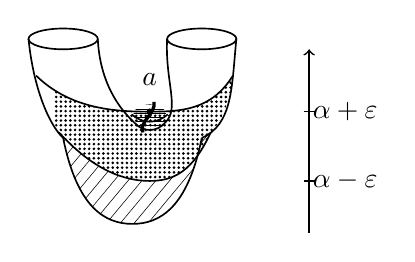
\begin{tikzpicture}[line width=0.6pt,scale=0.88]
  \draw (-0.05,1.65) .. controls (0.02,0.95) and (0.24,0.42) .. (0.45,0.22);
  \draw (0.95,1.65) .. controls (0.98,1.02) and (1.26,0.64) .. (1.48,0.44);
  \draw (1.95,1.65) .. controls (1.92,1.02) and (2.14,0.64) .. (1.92,0.44);
  \draw (2.95,1.65) .. controls (2.88,0.95) and (2.90,0.42) .. (2.45,0.22);
  \draw (0.45,0.22) .. controls (0.65,-0.78) and (1.05,-1.02) .. (1.45,-1.02)
        .. controls (1.85,-1.02) and (2.25,-0.78) .. (2.45,0.22);
  \draw (0.45,1.65) ellipse (0.5 and 0.15);
  \draw (2.45,1.65) ellipse (0.5 and 0.15);
  \draw (1.48,0.44) .. controls (1.60,0.30) and (1.80,0.30) .. (1.92,0.44);
  \draw (1.44,0.56) .. controls (1.60,0.42) and (1.80,0.42) .. (1.96,0.56);
  \draw (0.06,1.12) .. controls (0.57,0.62) and (1.25,0.60) .. (1.70,0.60)
        .. controls (2.15,0.60) and (2.59,0.62) .. (2.90,1.12);
  \draw (0.39,0.30) .. controls (0.90,-0.26) and (1.35,-0.40) .. (1.70,-0.40)
        .. controls (2.05,-0.40) and (2.32,-0.26) .. (2.58,0.30);
  \begin{scope}
    \clip (0.06,1.12) .. controls (0.57,0.62) and (1.25,0.60) .. (1.70,0.60)
          .. controls (2.15,0.60) and (2.59,0.62) .. (2.90,1.12)
          .. controls (2.87,0.85) and (2.78,0.50) .. (2.58,0.30)
          .. controls (2.32,-0.26) and (2.05,-0.40) .. (1.70,-0.40)
          .. controls (1.35,-0.40) and (0.90,-0.26) .. (0.39,0.30)
          .. controls (0.33,0.42) and (0.10,0.82) .. (0.06,1.12) -- cycle;
    \foreach \i in {0,...,38}
      \foreach \j in {0,...,22}
        \fill (0.35+0.068*\i,-0.48+0.068*\j) circle (0.021);
  \end{scope}
  \begin{scope}
    \clip (0.39,0.30) .. controls (0.90,-0.26) and (1.35,-0.40) .. (1.70,-0.40)
          .. controls (2.05,-0.40) and (2.32,-0.26) .. (2.58,0.30)
          -- (2.45,0.22) .. controls (2.25,-0.78) and (1.85,-1.02) .. (1.45,-1.02)
          .. controls (1.05,-1.02) and (0.65,-0.78) .. (0.45,0.22) -- cycle;
    \foreach \s in {-1.2,-1.0,...,2.6} \draw[very thin] (\s,-1.1) -- (\s+1.5,0.7);
  \end{scope}
  \begin{scope}
    \clip (1.50,0.44) .. controls (1.62,0.30) and (1.80,0.30) .. (1.90,0.44)
          -- (1.94,0.60) .. controls (1.80,0.74) and (1.60,0.74) .. (1.46,0.60) -- cycle;
    \foreach \h in {0.34,0.40,...,0.7} \draw[very thin] (1.44,\h) -- (1.96,\h);
  \end{scope}
  \draw[very thick] (1.60,0.30) .. controls (1.54,0.46) and (1.80,0.58) .. (1.76,0.74);
  \fill (1.70,0.60) circle (1.3pt);
  \node at (1.70,1.06) {$a$};
  \draw[->] (4.0,-1.15) -- (4.0,1.5);
  \draw (3.92,0.6) -- (4.08,0.6);
  \draw (3.92,-0.4) -- (4.08,-0.4);
  \node at (4.52,0.6) {$\alpha+\varepsilon$};
  \node at (4.52,-0.4) {$\alpha-\varepsilon$};
\end{tikzpicture}
\caption{}
\label{fig:crossing-ideas}
\end{minipage}\hfill
\begin{minipage}[b]{0.40\textwidth}
\centering
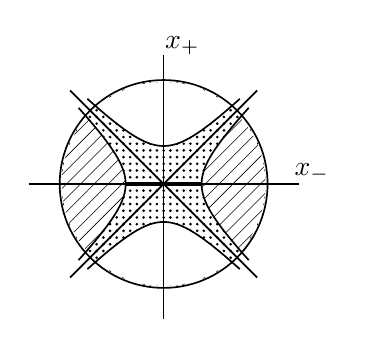
\begin{tikzpicture}[line width=0.6pt,scale=0.88]
  \draw (0,0) circle (1.5);
 \begin{scope}
  \clip (0,0) circle (1.48);
  \foreach \i in {0,...,30}
    \foreach \j in {0,...,30}
      \fill (-1.45+0.0967*\i,-1.45+0.0967*\j) circle (0.021);
 \end{scope}
  \fill[white] (49:1.47) arc[start angle=49,end angle=131,radius=1.47]
    -- plot[domain=0.965:-0.965] (\x,{sqrt(\x*\x+0.3)}) -- cycle;
  \fill[white] (-131:1.47) arc[start angle=-131,end angle=-49,radius=1.47]
    -- plot[domain=-0.965:0.965] (\x,{-sqrt(\x*\x+0.3)}) -- cycle;
  \fill[white] (41:1.47) arc[start angle=41,end angle=-41,radius=1.47]
    -- plot[variable=\y,domain=-0.965:0.965] ({sqrt(\y*\y+0.3)},\y) -- cycle;
  \fill[white] (139:1.47) arc[start angle=139,end angle=221,radius=1.47]
    -- plot[variable=\y,domain=0.965:-0.965] ({-sqrt(\y*\y+0.3)},\y) -- cycle;
  \begin{scope}
    \clip (41:1.47) arc[start angle=41,end angle=-41,radius=1.47]
      -- plot[variable=\y,domain=-0.965:0.965] ({sqrt(\y*\y+0.3)},\y) -- cycle;
    \foreach \s in {-2.4,-2.2,...,2.4} \draw[very thin] (\s,-1.6) -- (\s+3.2,1.6);
  \end{scope}
  \begin{scope}
    \clip (139:1.47) arc[start angle=139,end angle=221,radius=1.47]
      -- plot[variable=\y,domain=0.965:-0.965] ({-sqrt(\y*\y+0.3)},\y) -- cycle;
    \foreach \s in {-4.8,-4.6,...,0.2} \draw[very thin] (\s,-1.6) -- (\s+3.2,1.6);
  \end{scope}
  \draw[domain=-1.1:1.1,samples=25,smooth] plot (\x,{sqrt(\x*\x+0.3)});
  \draw[domain=-1.1:1.1,samples=25,smooth] plot (\x,{-sqrt(\x*\x+0.3)});
  \draw[variable=\y,domain=-1.1:1.1,samples=25,smooth] plot ({sqrt(\y*\y+0.3)},\y);
  \draw[variable=\y,domain=-1.1:1.1,samples=25,smooth] plot ({-sqrt(\y*\y+0.3)},\y);
  \draw (-1.35,-1.35) -- (1.35,1.35);
  \draw (-1.35,1.35) -- (1.35,-1.35);
  \draw (0,-1.95) -- (0,1.86);
  \draw (-1.95,0) -- (1.95,0);
  \node at (0.27,1.99) {$x_+$};
  \node at (2.14,0.16) {$x_-$};
  \draw[line width=1.6pt] (-0.55,0) -- (0.55,0);
\end{tikzpicture}
\caption{}
\label{fig:chart-model}
\end{minipage}
\end{figure}

\emph{$F$ 的构造。}

我们选取 $a$ 的邻域内的一个\trMorseChart{} $(U,h)$ 与一个充分小的 $\varepsilon>0$，使得 $f^{-1}([\alpha-\varepsilon,\alpha+\varepsilon])$ 是\trCompact{}的，并且 $U$ 包含以 $0$ 为中心、半径为 $\sqrt{2\varepsilon}$ 的球。\trDisk{} $D^k$ 是 $U$ 中由那些满足 $\|x_-\|^2<\varepsilon$ 与 $x_+=0$ 的 $(x_-,x_+)$ 所组成的子集。在\cref{fig:crossing-ideas}中，正如在\cref{fig:chart-model}中一样，\trSublevelSet{} $V^{\alpha-\varepsilon}$ 用斜细线标出，而 $f^{-1}([\alpha-\varepsilon,\alpha+\varepsilon])$ 则用点纹标出。\trCellular，亦即\trDisk{} $D^k$，是一条加粗的线段。

我们利用一个具有下列性质的 $\cC^\infty$ 函数 $\mu\colon[0,+\infty[\,\to[0,+\infty[$ 来构造函数 $F$：
\begin{itemize}
\item $\mu(0)>\varepsilon$；
\item 对 $s\ge 2\varepsilon$，$\mu(s)=0$；
\item 对每个 $s$，$-1<\mu'(s)\le 0$。
\end{itemize}

\begin{figure}[htbp]
\centering
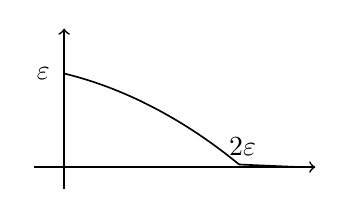
\begin{tikzpicture}[line width=0.6pt,scale=1.1]
  \draw[->] (0,-0.25) -- (0,1.6);
  \draw[->] (-0.35,0) -- (2.9,0);
  \draw (0,1.08) .. controls (0.75,0.9) and (1.45,0.5) .. (2.02,0.03);
  \draw (2.02,0.03) -- (2.72,0.0);
  \node at (-0.24,1.08) {$\varepsilon$};
  \node at (2.06,0.24) {$2\varepsilon$};
\end{tikzpicture}
\caption{函数 $\mu$}
\label{fig:mu-function}
\end{figure}

我们定义 $F$ 如下：
\[
F(x)=
\begin{cases}
f(x) & \text{若 } x\notin\Omega(a)\\[1ex]
\alpha-\|x_-\|^2+\|x_+\|^2-\mu\bigl(\|x_-\|^2+2\|x_+\|^2\bigr) & \text{若 } x=h(x_-,x_+)\text{。}
\end{cases}
\]
请注意，$F$ 对应 $\alpha+\varepsilon$ 的\trSublevelSet{}恰好就是 $f$ 的\trSublevelSet{} $V^{\alpha+\varepsilon}$。\footnote{译注：原书上式 $\|x_+\|^2$ 后无减号；按同页之 $F(a)=\alpha-\mu(0)$、$F|_{\mu=0}=f$ 及随后的导数 $dF=(-1-\mu')\,d\|x_-\|^2+(1-2\mu')\,d\|x_+\|^2$，疑漏排一负号；此处径改。——译者注}的确：
\begin{itemize}
\item 在 $\|x_-\|^2+2\|x_+\|^2\le 2\varepsilon$ 之外，我们有 $F=f$；
\item 在所述椭球的内部，我们有
\[
F(x)\le f(x)=\alpha-\|x_-\|^2+\|x_+\|^2
\le\alpha+\frac{1}{2}\|x_-\|^2+\|x_+\|^2\le\alpha+\varepsilon\text{。}
\]
\end{itemize}
此外，$F$ 的诸\trCriticalPoint{}与 $f$ 的相同，这是因为
\[
dF=\underbrace{\bigl(-1-\mu'(\|x_-\|^2+2\|x_+\|^2)\bigr)}_{<0}\,2x_-\cdot dx_-
+\underbrace{\bigl(1-2\mu'(\|x_-\|^2+2\|x_+\|^2)\bigr)}_{\ge 1}\,2x_+\cdot dx_+
\]
仅在 $x_-=x_+=0$ 处，也就是在 $a$ 处才为零。

我们现在知道
\[
F^{-1}([\alpha-\varepsilon,\alpha+\varepsilon])\subset f^{-1}([\alpha-\varepsilon,\alpha+\varepsilon])\text{；}
\]
特别地，这个区域是\trCompact{}的。此外，它不含 $F$ 的任何\trCriticalPoint：唯一可能的候选是 $a$，但是
\[
F(a)=\alpha-\mu(0)<\alpha-\varepsilon\text{。}
\]
由此可知，$F^{-1}(\,]{-\infty},\alpha+\varepsilon]\,)$ 是 $V^{\alpha+\varepsilon}$ 的一个\trDeformationRetract{}核。设 $H$ 是\cref{fig:crossing-ideas}中带水平细线的部分（在\cref{fig:chart-H}中它是清楚的），也就是说，它是 $F^{-1}(\,]{-\infty},\alpha-\varepsilon]\,)-V^{\alpha-\varepsilon}$ 的闭包。特别地，我们有
\[
F^{-1}(\,]{-\infty},\alpha-\varepsilon]\,)=V^{\alpha-\varepsilon}\cup H\text{。}
\]

\emph{收缩。}

我们沿\cref{fig:retraction}中所标出的那些箭头来定义这个收缩。明确地说，$r_t$ 在 $\Omega(a)$ 之外是恒同映射，而我们（为了记号简便）把 $r_t$ 定义在 $U$ 上（而非 $\Omega(a)$ 上）：

\begin{figure}[htbp]
\begin{minipage}[b]{0.46\textwidth}
\centering
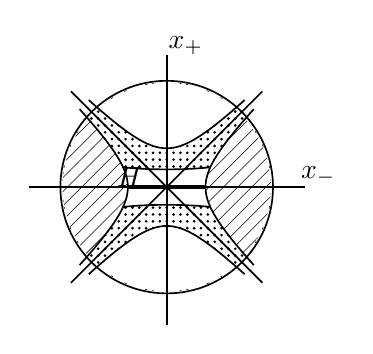
\begin{tikzpicture}[line width=0.6pt,scale=0.9]
  \draw (0,0) circle (1.5);
 \begin{scope}
  \clip (0,0) circle (1.48);
  \foreach \i in {0,...,30}
    \foreach \j in {0,...,30}
      \fill (-1.45+0.0967*\i,-1.45+0.0967*\j) circle (0.021);
 \end{scope}
  \fill[white]
    (-0.62,0.28) .. controls (-0.25,0.24) and (0.25,0.24) .. (0.62,0.28)
    -- plot[variable=\y,domain=0.28:-0.28] ({sqrt(\y*\y+0.3)},\y)
    .. controls (0.25,-0.24) and (-0.25,-0.24) .. (-0.62,-0.28)
    -- plot[variable=\y,domain=-0.28:0.28] ({-sqrt(\y*\y+0.3)},\y) -- cycle;
  \fill[white]
    (41:1.47) arc[start angle=41,end angle=-41,radius=1.47]
    -- plot[variable=\y,domain=-0.95:0.95] ({sqrt(\y*\y+0.3)},\y) -- cycle;
  \fill[white]
    (139:1.47) arc[start angle=139,end angle=221,radius=1.47]
    -- plot[variable=\y,domain=0.95:-0.95] ({-sqrt(\y*\y+0.3)},\y) -- cycle;
  \fill[white] (49:1.47) arc[start angle=49,end angle=131,radius=1.47]
    -- plot[domain=0.965:-0.965] (\x,{sqrt(\x*\x+0.3)}) -- cycle;
  \fill[white] (-131:1.47) arc[start angle=-131,end angle=-49,radius=1.47]
    -- plot[domain=-0.965:0.965] (\x,{-sqrt(\x*\x+0.3)}) -- cycle;
  \begin{scope}
    \clip (41:1.47) arc[start angle=41,end angle=-41,radius=1.47]
      -- plot[variable=\y,domain=-0.965:0.965] ({sqrt(\y*\y+0.3)},\y) -- cycle;
    \foreach \s in {-2.4,-2.2,...,2.4} \draw[very thin] (\s,-1.6) -- (\s+3.2,1.6);
  \end{scope}
  \begin{scope}
    \clip (139:1.47) arc[start angle=139,end angle=221,radius=1.47]
      -- plot[variable=\y,domain=0.965:-0.965] ({-sqrt(\y*\y+0.3)},\y) -- cycle;
    \foreach \s in {-4.8,-4.6,...,0.2} \draw[very thin] (\s,-1.6) -- (\s+3.2,1.6);
  \end{scope}
  \draw[domain=-1.1:1.1,samples=25,smooth] plot (\x,{sqrt(\x*\x+0.3)});
  \draw[domain=-1.1:1.1,samples=25,smooth] plot (\x,{-sqrt(\x*\x+0.3)});
  \draw[variable=\y,domain=-1.1:1.1,samples=25,smooth] plot ({sqrt(\y*\y+0.3)},\y);
  \draw[variable=\y,domain=-1.1:1.1,samples=25,smooth] plot ({-sqrt(\y*\y+0.3)},\y);
  \draw (-0.62,0.28) .. controls (-0.25,0.24) and (0.25,0.24) .. (0.62,0.28);
  \draw (-0.62,-0.28) .. controls (-0.25,-0.24) and (0.25,-0.24) .. (0.62,-0.28);
  \draw (-1.35,-1.35) -- (1.35,1.35);
  \draw (-1.35,1.35) -- (1.35,-1.35);
  \draw (0,-1.95) -- (0,1.86);
  \draw (-1.95,0) -- (1.95,0);
  \node at (0.27,1.99) {$x_+$};
  \node at (2.14,0.16) {$x_-$};
  \draw[line width=1.6pt] (-0.55,0) -- (0.55,0);
  \node at (-0.52,0.14) {$H$};
\end{tikzpicture}
\caption{}
\label{fig:chart-H}
\end{minipage}\hfill
\begin{minipage}[b]{0.46\textwidth}
\centering
\begin{tikzpicture}[line width=0.6pt,scale=1.0]
  \draw (0,1.0) .. controls (1.0,0.66) and (2.2,0.66) .. (3.2,1.0);
  \draw (0,-0.1) .. controls (1.0,0.26) and (2.2,0.26) .. (3.2,-0.1);
  \draw (0,1.0) .. controls (-0.14,0.45) .. (0,-0.1);
  \draw (3.2,1.0) .. controls (3.34,0.45) .. (3.2,-0.1);
  \foreach \x in {0.30,0.56,...,2.90}
    \draw[->] (\x,{0.745+0.255*((\x-1.6)/1.6)^2-0.02}) -- (\x,0.50);
  \foreach \x in {0.30,0.56,...,2.90}
    \draw[->] (\x,{0.170-0.270*((\x-1.6)/1.6)^2+0.02}) -- (\x,0.36);
  \draw[very thick] (0.22,0.42) -- (2.98,0.42);
  \node at (1.6,1.28) {$H$};
  \node (p3) at (-0.75,1.2) {区域~3};
  \draw[->] (p3) -- (0.12,0.92);
  \node (p1) at (1.73,-0.85) {\small 区域~1};
  \draw[->] (p1) -- (1.73,0.30);
  \node (p2) at (2.75,-0.5) {区域~2};
  \draw[->] (p2) -- (2.42,0.1);
\end{tikzpicture}
\caption{}
\label{fig:retraction}
\end{minipage}
\end{figure}

\begin{itemize}
\item 在区域 1（\cref{fig:retraction}）上，亦即在 $\|x_-\|^2\le\varepsilon$ 上，
\[
r_t(x_-,x_+)=(x_-,t x_+)\text{。}
\]
\item 在区域 2——它由 $\varepsilon\le\|x_-\|^2\le\varepsilon+\|x_+\|^2$ 所定义——上，我们令
\[
r_t(x_-,x_+)=(x_-,s_t x_+)\text{，}
\]
其中
\[
s_t=t+(1-t)\frac{\sqrt{\|x_-\|^2-\varepsilon}}{\|x_+\|}
\]
便是使这些公式连续的恰当数值。\footnote{译注：原书此处“区域 2”条件印作 $\varepsilon\le\|x_-\|^2\le\varepsilon\|x_+\|^2$；由 $s_t$ 式须在边界 $\|x_-\|^2=\varepsilon+\|x_+\|^2$ 处连续、且与区域 3 的条件 $\|x_+\|^2+\varepsilon\le\|x_-\|^2$ 互证，右端疑漏排加号；此处径改。——译者注}
\item 在区域 3——它对应于 $V^{\alpha-\varepsilon}$，并且满足 $\|x_+\|^2+\varepsilon\le\|x_-\|^2$——上，我们干脆取 $r_t=\operatorname{Id}$。
\end{itemize}
\end{proof}
